% SPDX-License-Identifier: CC-BY-4.0
% Copyright (c) 2026 Jonathan Yantis. Author-review research draft.
\documentclass[11pt,letterpaper]{article}
\usepackage[margin=0.78in]{geometry}
\usepackage[T1]{fontenc}
\usepackage{lmodern,microtype,amsmath,amssymb,booktabs,array,ragged2e,xcolor,tikz,pgfplots,enumitem,fancyhdr,xurl}
\usetikzlibrary{arrows.meta,positioning,calc}
\pgfplotsset{compat=1.18}
\usepackage[colorlinks=true,allcolors=ink]{hyperref}
\definecolor{ink}{HTML}{24465B}\definecolor{pale}{HTML}{EDF2F3}\definecolor{amber}{HTML}{A85F2B}
\setlength{\parindent}{0pt}\setlength{\parskip}{4pt}\setlength{\headheight}{14pt}\setlength{\emergencystretch}{2em}
\setlist{nosep,leftmargin=1.4em}\widowpenalty=10000\clubpenalty=10000
\newcolumntype{L}[1]{>{\RaggedRight\arraybackslash}p{#1}}
\newcommand{\ns}{\,\mathrm{ns}}\newcommand{\us}{\,\mu\mathrm{s}}\newcommand{\ms}{\,\mathrm{ms}}
\newcommand{\src}[1]{\nolinkurl{#1}}
\pagestyle{fancy}\fancyhf{}\fancyhead[L]{\small PToB: timing tails and multipath}\fancyhead[R]{\small AUTHOR-REVIEW DRAFT -- 26 October 2026}\fancyfoot[C]{\thepage}
\hypersetup{pdftitle={Reducing Timing Tails and Multipath Sensitivity in an Operating BLE Precision Mesh},pdfauthor={Jonathan Yantis}}
\begin{document}
\begin{center}
{\LARGE\bfseries Reducing Timing Tails and Multipath Sensitivity\\[3pt] in an Operating BLE Precision Mesh}\par
\vspace{7pt}Jonathan Yantis\quad\textit{Independent researcher}\par
26 October 2026\quad Research draft for author review; not submitted or peer reviewed
\end{center}
\vspace{-5pt}
\begin{abstract}\noindent
Wireless clock synchronization has long improved precision by removing uncertain software delay from the timestamp path. Multipath leaves a different problem: the receiver detects a composite waveform, while packet loss can age an otherwise correct clock model. This paper connects those established problems to PToB's operating Bluetooth Low Energy mesh. It reviews event association, capture, clock bridging, channel-aware frequency fitting, bounded steering and source ownership, then proposes placement, instrumentation, estimator and scheduling tests on existing Nordic nRF52840 and ESP32-S3 targets. Historical W12 and N30 observations retain distinct populations, missing records and calibration scopes; their tails do not establish multipath causation. Analytical examples expose channel-mix confounding and stale-correction costs. A falsifiable programme combines offline replay with future common-reference tests, frozen images and held-out placements. Improved capture resolution neither identifies the first RF path nor establishes calibrated UTC/output accuracy.
\end{abstract}
\vspace{-5pt}
\section{Scope, evidence and the problem to solve}
PToB distributes time over authenticated BLE periodic advertising. The argument follows three questions: what physical event does a receiver observe, which uncertainties can the current implementation remove, and which experiments distinguish the remaining causes? This implementation review uses source checkpoint \src{ea70b7f5b5bd}, with exact file hashes in the edition receipt [1]. Historical observations, analytical illustrations and proposed changes remain distinct; no new RF campaign is reported.

The normal RC7 interval is $50\times1.25\ms=62.5\ms$, or 16 events/s [1,2]. This is a scheduled event cadence, not a measured application latency or clock error. A valid clock map is evaluated against a continuously running counter between packets. Loss can increase its age or remove permission; a read need not wait for the next advertisement.

\begin{center}\small
\begin{tabular}{L{.31\linewidth}L{.23\linewidth}L{.37\linewidth}}\toprule
Separate historical population & Eligible / opportunities & Bias-inclusive RMS; maximum $|e|$\\\midrule
W12 PPS, 24 October [5] & 522 / 600 logged & $60.328\ns$; $180\ns$\\
Downstream PPS, same study & 451 / 600 logged & $61.922\ns$; $211\ns$\\
Selected TX at downstream RX & 58 / 120 selected & $108.306\ns$; $226\ns$\\
N30 PPS, 22 October [6] & 657 / 660 nominal & $166.590\ns$; $1591\ns$\\\bottomrule
\end{tabular}
\end{center}\vspace{-5pt}
W12 used firmware 0.2.10 with T096 0.15.169 and frozen path adjustments; GNSS was a witness, not BLE feedback. Its 78 source-unavailable records remain. Downstream retained 109 no-map, 36 expired and four reference-ineligible records; selected TX retained 61 unmatched and one unbracketed record. N30 retained three invalids, no nominal missing and four eligible excursions above $1\us$, whose cause was not isolated. The fixed window later selected a 51016 ns profile; it cannot validate that retuning. Its separate 48/64 second-board transfer is not pooled. Calibration, training and validation are not interchangeable; later source changes inherit no qualification from these windows.

{\footnotesize Copyright \copyright\ 2026 Jonathan Yantis. Original paper, LaTeX, figures and derived analysis: \href{https://creativecommons.org/licenses/by/4.0/}{CC BY 4.0}. Ordinary documentation and executable verifier: MIT. Cited works retain their terms.}
\newpage
\section{Multipath in context: propagation and synchronization}
\subsection{A longstanding radio problem reaches a finer timing budget}
Indoor multipath predates BLE. Saleh and Valenzuela's 1987 office-building pulse measurements characterized delayed arrivals [13]: a room presents multiple paths, not one geometrical distance. Those measurements do not calibrate today's BLE boards. TI's later diversity work [8] addresses the related reception problem: different positions, antennas or frequencies can experience different fading in the same environment.

For interpretation, a locally static channel can be written schematically as
\[
 r_k(u)=\sum_{\ell=0}^{m} a_{\ell,k}\,s(u-\tau_\ell)+n_k(u),
\]
where $s$ is the transmitted waveform, $\tau_\ell$ are path delays and complex $a_{\ell,k}$ include amplitude and phase at channel $k$. The receiver sees their superposition. Changing frequency or moving a reflector can change that sum without changing the clocks. A direct component can coexist with strong reflections; obstruction can attenuate it below useful detectability. Non-line-of-sight placement and multipath are related conditions, not interchangeable labels.

Two consequences matter for a timing mesh. First, a successfully decoded packet can have an environment-dependent detector reference: the digital timestamp marks the receiver's response to the composite signal, not a separately measured first path. A CRC establishes packet integrity, not timing unbiasedness. Second, destructive fading can prevent reception altogether. That loss increases correction age, may trigger holdover or source withdrawal, and can produce a later clock excursion through oscillator prediction or handover. This indirect route from RF conditions to a tail does not require a microsecond of extra propagation.

The distinction explains why amplitude diversity and frequency hopping can improve delivery without proving an improvement in phase accuracy. It also explains why the strongest RSSI, smallest residual and earliest callback are not equivalent observations. Commodity packet-event captures expose none of the full impulse response needed to resolve this ambiguity. This paper therefore treats environmental timing bias and loss-induced aging as separate hypotheses, with separate observables.

\subsection{What earlier synchronization systems learned to remove}
Reference-Broadcast Synchronization (RBS, 2002) compared receivers observing the same broadcast, removing the sender's send/access uncertainty from their comparison [14]. Its analysis treated propagation differences of tens of nanoseconds as small within a microsecond-scale budget. The architectural insight remains useful, but that approximation needs reconsideration when a timing study evaluates errors of order $100\ns$. Shared transmitter delay can cancel between receivers while unequal paths and receiver delays remain.

FTSP (2004) combined MAC-level timestamps with clock-skew estimation and flooding [10]. CheepSync (2015/2016) carried low-level timestamping and drift compensation into heterogeneous BLE advertising devices [16]. Together these works establish why timestamp location, event identity and oscillator estimation deserve attention before attributing residual error to the channel. Their protocols, endpoints and error populations differ from PToB's; their reported averages cannot rank this mesh's tails.

PToB follows this lineage through exact event joins, explicit capture boundaries and causal models. The remaining task is diagnostic: define the delivered quantities, locate each uncertainty, and test competing explanations. Precisely capturing a biased detector event and delivering an accurate event too late require different remedies.
\newpage
\section{Measure different tails at explicit endpoints}
Define a run's nominal opportunities before collection: scheduled RF events for link delivery, declared reference edges for PPS, and a fixed sampling grid for clock service. These denominators differ. At opportunity $i$, record the event time $t_i$, matching correction availability $a_i$, and actual clock-map activation $v_i$ in a declared common coordinate. Then $L_i=a_i-t_i$ measures event-to-correction delivery; $v_i-a_i$ measures application delay. Neither includes an arbitrary application's transport unless explicitly instrumented.

At query time $t$, let $j(t)$ be the newest physical observation actually incorporated into the delivered model. Correction age is $A(t)=t-t_{j(t)}$. Delivered error is $e(t)=\widehat T(t)-T_{\rm ref}(t)$ at the specified software read or electrical PPS endpoint. Score internal pre-update prediction residuals separately. A software map, GPIO edge and USB/host result have different delays and uncertainty budgets.

For $n$ eligible residuals, report signed mean, uncentered RMS, maximum absolute error and nearest-rank absolute quantiles:
\[
 Q_p(|e|)=|e|_{(\lceil pn\rceil)},\qquad
 R=\sqrt{n^{-1}\sum_i e_i^2},\qquad R^2=\overline e^{\,2}+\sigma_{\rm population}^2.
\]
Always publish $n/N$ and exclusion reasons alongside conditional statistics. P99 clock error is not P99 delivery latency. Define service availability on all $N$ query opportunities, separately from reference scoreability; an invalid witness does not prove absent service. Report the longest consecutive loss/unavailable burst, elapsed outage duration, and recovery time from an observed perturbation to the first interval meeting a predeclared sustained criterion. Right-censor recovery if the run ends first. Sampled status cannot establish continuous availability between samples.

\begin{center}
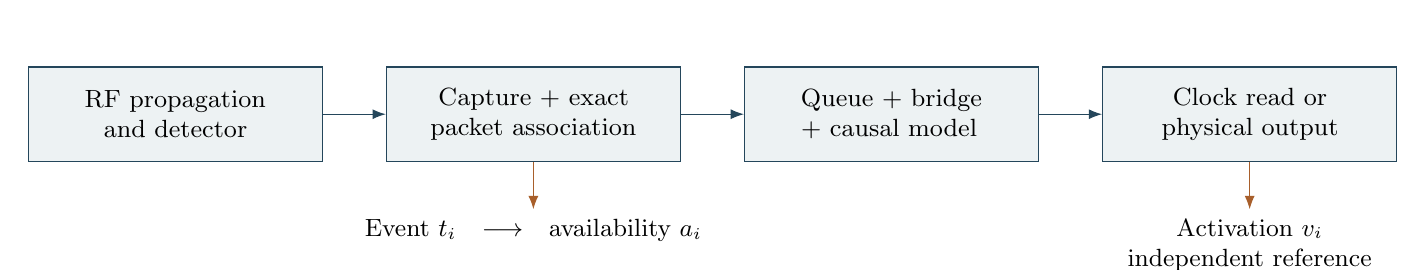
\begin{tikzpicture}[>=Latex,font=\small,box/.style={draw=ink,fill=pale,text width=35mm,align=center,minimum height=12mm},node distance=8mm]
\node[box](rf){RF propagation\\and detector};
\node[box,right=of rf](cap){Capture + exact\\packet association};
\node[box,right=of cap](map){Queue + bridge\\+ causal model};
\node[box,right=of map](out){Clock read or\\physical output};
\draw[->,ink](rf)--(cap);\draw[->,ink](cap)--(map);\draw[->,ink](map)--(out);
\node[below=6mm of cap,align=center](a){Event $t_i$\quad$\longrightarrow$\quad availability $a_i$};
\node[below=6mm of out,align=center](b){Activation $v_i$\\independent reference};
\draw[->,amber](cap.south)--(a.north);\draw[->,amber](out.south)--(b.north);
\end{tikzpicture}
\end{center}\vspace{-6pt}
{\small\textbf{Figure 1.} Distinct boundaries to instrument. RF bias can survive perfect capture; queue delay can age a correct capture. Output error requires an independent endpoint witness. Arrows are conceptual, not measured delays.}

\subsection{An error budget is a diagnostic model, not a calibration}
A useful decomposition is
\[
 e(t)=b_{\rm path}+b_{\rm TX/RX}+d_{\rm env}(t,k)+e_{\rm assoc}
       +e_{\rm bridge}+e_{\rm model}(t,A)+e_{\rm output}-e_{\rm ref}.
\]
Here $k$ is RF channel; terms may be coupled or unobservable. Do not add their RMS values in quadrature without justified covariance and bias treatment. Unknown endpoint/reference bounds remain unknown. Pure excess distance $\Delta\ell$ gives $\Delta\ell/c$: 1 m is $3.336\ns$ and 30 m is $100.069\ns$. Thus a microsecond excursion alone does not identify a long reflected path: both the direct detector effect and indirect aging route from Section 2 must compete with association, scheduling, warm-up and reference errors. Common-reference agreement can also hide common-mode error.
\newpage
\section{What the current implementation actually mitigates}
\textbf{Capture and exact association.} T096 routes RADIO ADDRESS through PPI to TIMER3 CC1; the owner preserves that capture and checks completion, CRC on RX, payload class, event and channel [1,3]. PPI removes CPU interrupt arrival from that latch. It does not measure the first arriving ray or establish equal transmit/receive detector delays. A later software callback identifies delivery, not the original radio edge. FTSP's original MAC timestamping and skew compensation provide relevant precedent [10]; their platform results do not transfer numerically to PToB.

The selected fine W12/N30 paths instead use a continuous 80 MHz capture counter, exact retained-packet joins and an empirical RX-marker convention [1,7]. Resolution is $12.5\ns$; delivered coordinates round to $50\ns$. Neither is calibrated accuracy. Missing, ambiguous, overwritten, late or unsupported associations remain unavailable. Clock incarnation and wrap extension must survive packet silence. SS3 remains a distinct profile; fine-path availability and wiring require target checks. W12, SS3 and N30 are RC targets, not qualified GMs. N30/SS3 have no GNSS input; W12 GNSS requires an explicit board/profile selection.

\textbf{Clock bridges and model causality.} Narrow local read brackets enclose the observation of another counter; preserve both bounds, clock domains and epochs. ESP-IDF's driver documentation distinguishes capture clocks, power-management locks and cache-safe interrupt operation [4]. Those software contracts do not characterize an RF endpoint. Current fine paths freeze a prediction at capture before its unseen correction can train the model. Re-evaluating that past edge using a later fitted map would conceal causal error. Model generation and activation time must accompany every comparison.

\textbf{Channel-aware rate fitting.} Current fine fitting retains up to 64 physical points, including the 16 Hz opportunities, and estimates rate from repeated observations within channel [1]. In the diagnostic model
\[
 r_i=\phi+f x_i+b_{k_i}+\epsilon_i,\qquad
 \widehat f=\frac{\sum_k\sum_{i\in k}(x_i-\bar x_k)(r_i-\bar r_k)}
 {\sum_k\sum_{i\in k}(x_i-\bar x_k)^2},
\]
fixed channel offsets cancel from the rate estimate. For times $(0,1,2,3)$ s, channels $(a,a,b,b)$ and residuals $(0,20,140,160)\ns$, pooled regression gives $60\ns$/s while within-channel regression gives the true illustrative $20\ns$/s. The difference comes from a $100\ns$ channel offset and changing mix, not oscillator acceleration. These are analytical values. Repeated-channel support and adequate time span are necessary; if channel delay changes with time, rate remains confounded. Centering does not calibrate $b_k$, remove phase bias or prove multipath mitigation. All causal errors and full tails are scored independently of fitting selection.

\textbf{Steering, ownership and scheduling.} Phase, frequency and bounded acceleration handling serve different purposes. Bounded phase slew limits abrupt delivered-map movement, but prolongs response to a genuine phase change. Source expiry, authenticated scope, stable parent selection and actual controller ownership prevent stale or foreign corrections from acquiring authority. Current W12 processing shares an eight-report precision budget across control boundaries, with fresh time reads after yielding calls [1]. This bounds report count, not worst-case wall time. Queue overflow, late callbacks, failed drains and map withdrawal still need explicit accounting. Successful host tests establish software behavior only.

W12 BLE50 is client-only; BLE100 relaying uses programmed/estimated TX timing with unknown RF bounds. T096's nominal LE1M endpoint and S3's programmed packet-start reference differ by the preamble/access-address duration, $40\us$ [2,7]. Converting a reference convention removes that nominal mismatch, not controller or propagation jitter. The frozen aggregate per-path calibration cannot identify its separate TX and RX components.
\newpage
\section{Practical RF mitigation and candidate tail controls}
\subsection{Start with installation geometry and retain diversity}
Improve direct-path visibility where practical: raise antennas away from floors, metal surfaces, enclosures, power/USB leads and nearby bodies; record antenna orientation, polarization, board mounting and cable routing. Avoid a universal clearance distance: the board antenna, ground plane and enclosure matter [9]. Compare a small spatial grid and controlled orientations without changing software. At an illustrative 2.44 GHz, $\lambda=c/f=12.287$ cm; $\lambda/2=6.143$ cm is a useful sweep scale, not a guaranteed decorrelation distance. Include multiple heights and preserve an attainable installation choice rather than selecting one lucky sample.

TI's diversity study addresses packet reception using alternate antennas/frequencies on other radios [8]. It motivates tests of fading sensitivity, not a nanosecond timing claim. Strong RSSI can include strong reflections; it is not a first-path quality measurement. Analyze signed phase, tails, age and loss by channel and RSSI jointly. A minimum observed residual is also affected by clock/reference bias, noise and selection; it is not a direct-path estimator.

Retain normal frequency diversity while gathering per-channel diagnostics. Periodic-advertising channel-map updates have advertiser/controller ownership and synchronization rules [2]; a receiver cannot independently blacklist channels and assume the train follows. Before proposing map changes, prove the target stack exposes a supported control path for that train, and test its scheduling/association impact. No reviewed PToB user API for this intervention is asserted here. Restricting channels may reduce repeated-channel fit delay yet concentrate interference and environmental bias. Separate primary discovery channels from the secondary train's channels in logs.

Switched antenna diversity requires suitable RF routing/switches, controller timing and per-path calibration. It is not a software option established on these installed boards. Two receivers at separated placements are a future diagnostic comparison, not coherent antenna combining. Current targets supply neither a wideband channel impulse response nor a qualified Bluetooth Channel Sounding implementation. A newer Core specification does not grant those capabilities to existing silicon.

\subsection{Candidates to test without discarding real tails}
\textbf{Bound work and expose delay.} Add bounded, nonblocking telemetry for queue high-water marks, overwrite/drop reasons, capture-to-worker time, bracket width, model generation/activation, source age and owner transitions. Cap elapsed work as well as record count; prioritize capture/precision before console, display and admission work. Avoid logging inside timing-critical regions. Compare instrumentation enabled/disabled to detect observer effects. A throughput gain fails if it increases expiry or hides dropped opportunities.

\textbf{Prospective robust weighting.} Replay a bounded-influence or variance-weighted rate/phase estimator with weights selected from past data and declared channel/age support. Compare it with the current fitter on identical chronological opportunities. Log raw innovation, weight, refusal and delivered prediction for every point. Robustness may reduce sensitivity to corrupted training samples but can delay real source steps or warm-up tracking. Scoring includes valid large errors regardless of weight; rejected physical samples still affect availability and age. Do not trim validation residuals or tune against the held-out run.

\textbf{Qualified holdover and stable selection.} Withdraw timing when inherited permission or a validated forecast expires. A good oscillator fit cannot renew source authority. Compare parent hysteresis/dwell with controlled handover, keeping root/boot/epoch/path fences and actual drain ownership. More smoothing can reduce jitter while increasing recovery time; more RF listening can reduce correction age while increasing power and scheduler contention. None of these tradeoffs is settled by a lower displayed RMS.
\newpage
\section{A falsifiable validation programme on existing hardware}
Run offline replay/host checks first. All matrix tests are proposed and unrun. Future hardware blocks require separate authorization, frozen image, exact board identity, PHY/PDU, endpoint, calibration and source path. Use an independent common-reference witness with declared cable/GPIO/instrument uncertainty. Label internal-only results accordingly. Retain baseline blocks and randomize intervention order.

\begin{center}\small
\renewcommand{\arraystretch}{1.16}\setlength{\tabcolsep}{4pt}
\begin{tabular}{L{.09\linewidth}L{.255\linewidth}L{.28\linewidth}L{.285\linewidth}}\toprule
Priority / test & Hypothesis; controlled change & Instrumentation; held constant & Observable, decision; failure meaning\\\midrule
P0\newline Replay & Association, wrap or activation races create tails. Inject delayed/duplicate callbacks, silence, changed epochs and old-owner queues. & Actual host matcher/clock code; synthetic identities, original expiry, chronology and frozen predictions. & Wrong-scope/ambiguous joins refused; no future-model score or expiry extension. Any violation blocks the candidate.\\
P1\newline Load & Queue/scheduler delay dominates aging. Vary CPU, USB/console, display and admission traffic individually. & Same image, calibration, placement, reference; queue/worker/owner telemetry; paired instrumentation-off blocks. & Compare latency/age P99, error tails, loss bursts and service. Delay shifts with fixed geometry support scheduling; no shift weakens that hypothesis.\\
P1\newline RF & Geometry changes channel-dependent fading/bias. Compare LOS, reflective LOS, obstructed/NLOS, spatial/orientation and moving-person blocks. & Same image, rate, power, load, reference routing; log geometry, channel, RSSI, CRC/loss and independent RF occupancy. & Repeatable environment--channel effects after load control support sensitivity. Nonrepeatability or only occupancy-linked loss defeats a multipath-only explanation.\\
P2\newline Drift & Warm-up/temperature increases forecast error. Compare cold/warm starts and temperature plateaus. & Same geometry, reference, load; independently measured temperature, rates, brackets and age. & Error versus age/rate must fit the declared forecast. Exceedance withdraws the holdover budget; correlation alone is not causality.\\
P2\newline Path & Bias is stable only within declared scope. Compare direct/relay, then held-out units/placements. & Exact source/boot/path, frozen adjustments; common-reference path-delay check. No validation refit. & Retain signed bias and all tails. Transferred bias beyond frozen uncertainty falsifies portability; no retrospective repair.\\
P2\newline Recovery & Stable ownership/admission limits outages. Apply bounded source withdrawal/change and return. & Frozen images, known sources, original leases/drains; independent continuity and activation/owner trace. & Record outage, censored recovery and excursion. Stale permission, owner overlap or missed deadline fails despite eventual lock.\\
P3\newline Estimator & Prospective weighting reduces contamination without concealing service errors. & Paired chronological replay; frozen settings, held-out blocks, identical records and opportunity grid. & Require preregistered tail improvement and availability/recovery noninferiority. Better fit with worse delivered tails rejects the candidate.\\\bottomrule
\end{tabular}
\end{center}\vspace{-4pt}
\textbf{Decision contract.} Preregister application budget $B$, tail/latency improvement margin $\Delta$, allowable availability change and maximum recovery $R$. Require a paired run/block-level uncertainty interval favoring the primary tail metric by $\Delta$, with availability/recovery noninferiority. Correct exploratory multiple comparisons or validate selections in fresh blocks. Preserve every failure and offending tail.
\newpage
\section{Aging, rare events and honest inference}
\subsection{An analytical holdover example, not a device bound}
If initial absolute error is bounded by $E_0$, residual rate by $Y$ and rate change by $D$, a conditional forecast is
\[
 |e(t)|\le E_0+Y A(t)+\tfrac12 D A(t)^2.
\]
Every quantity needs a validated scope. With hypothetical $E_0=100\ns$, $Y=20\ns$/s and $D=2\ns$/s$^2$, ages 1, 5 and 10 s give 121, 225 and $400\ns$. A hypothetical 0.5 ppm residual rate instead contributes $500\ns$/s, giving $2600\ns$ at 5 s even with $D=0$. If any required bound is unknown, these expressions do not provide a qualified service bound.

\begin{center}
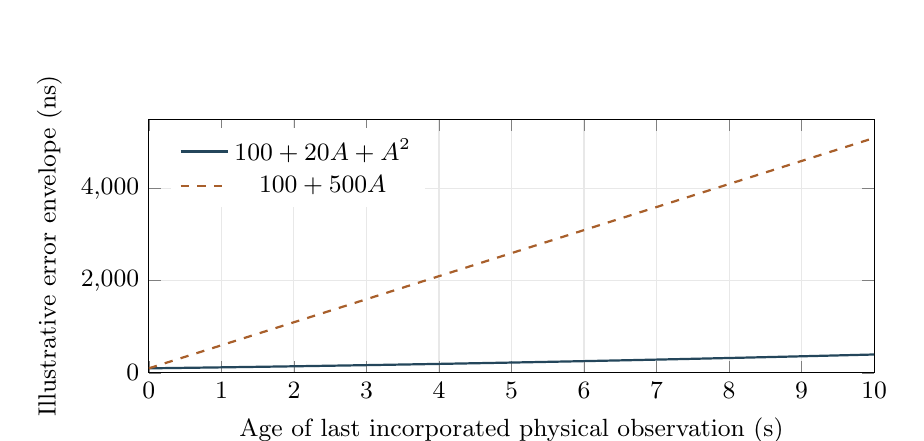
\begin{tikzpicture}
\begin{axis}[width=.89\linewidth,height=48mm,xmin=0,xmax=10,ymin=0,ymax=5500,
 xlabel={Age of last incorporated physical observation (s)},ylabel={Illustrative error envelope (ns)},
 tick label style={font=\small},label style={font=\small},legend style={font=\small,at={(.03,.97)},anchor=north west,draw=none},grid=major,grid style={gray!18}]
\addplot[ink,thick,domain=0:10,samples=51]{100+20*x+x*x};\addlegendentry{$100+20A+A^2$}
\addplot[amber,thick,dashed,domain=0:10]{100+500*x};\addlegendentry{$100+500A$}
\end{axis}
\end{tikzpicture}
\end{center}\vspace{-8pt}
{\small\textbf{Figure 2.} Analytical sensitivity to correction age under two declared hypothetical oscillator assumptions. No curve is fitted to PToB hardware. Source permission can expire before either envelope reaches an application budget.}

Ten consecutive missed 16 Hz events span $625\ms$ of scheduled opportunities. Immediately before the following successful event, the last successful event can be $687.5\ms$ old, plus correction processing. A count of losses alone is not an age measurement. Under the additional ideal assumptions of independent loss probability $p=0.1$ per event, every delivered event immediately usable and no expiry, the post-opportunity count of consecutive misses has $P(K\ge k)=p^k$. Its P99 is one missed interval ($62.5\ms$). Real burst loss, asynchronous queries, delayed corrections and source withdrawal invalidate that convenient model.

\subsection{Confidence requires opportunities and independent information}
With independent, identically distributed Bernoulli exceedances, zero in $n$ trials gives the exact one-sided 95\% upper probability $1-0.05^{1/n}$, derived from $P(0)=(1-p)^n$. At $n=600$ this is $0.498\%$, not zero; excluding a probability of $10^{-4}$ requires at least $29\,956$ independent trials, about $31.204$ min at 16 Hz. This is an ideal sample-size illustration, not a recommended campaign duration or a guarantee for correlated clocks. A 1 Hz PPS stream has a different count.

For measured quantiles, use binomial order-statistic intervals only when independence/stationarity is defensible. Serial correlation, overlapping model fits and common source changes reduce independent information. Use repeated runs and blocks longer than the observed dependence, report run-level dispersion, and use a declared block-resampling analysis for paired comparisons. Short runs may contain too few tail events to resolve P99.9; the maximum is only an observed maximum. Preserve startup, invalid, missing, rejected and source-unavailable classes and each phase's denominator, even when primary steady-state scoring is separately preregistered. A clean final window cannot replace the full run.
\newpage
\section{Priorities, limits and reproducibility}
The historical lesson is to remove uncertainty where its cause is observable. RBS shortened the uncertain comparison path; FTSP and BLE synchronization studies improved timestamping and drift estimation. PToB's exact joins and channel-aware causal fitter address the same class of problems at different boundaries. The remaining experiment is not simply to show a smaller RMS: it is to determine whether a tail follows the detector/geometry, delayed processing, aging, model activation or source transition.

\textbf{First, establish causal observability.} Preserve exact joins, clock/map generations and original permission under replay faults; measure queue age and activation. \textbf{Second, compare workload and placement.} P1 paired blocks distinguish controller/CPU effects from environmental sensitivity, retaining interference evidence and per-channel distributions. \textbf{Third, validate control changes.} Test weighting, holdover and selection on held-out units, rooms and transitions, requiring availability/recovery as well as tail improvement. Recalibration creates a new scoped experiment.

An important limit is identifiability, not just sample count. Freris, Graham and Kumar showed for affine-clock network models that clock offsets and unknown directional link delays cannot all be recovered uniquely from timestamp exchanges without additional structure [15]. A one-way observation illustrates the issue: $z=\theta+d$ is unchanged by $\theta'=\theta+\delta$, $d'=d-\delta$, whenever the alternative delays remain admissible. More observations can estimate rate and variation while leaving a fixed offset/delay ambiguity. PToB's frozen aggregate adjustments are therefore scoped empirical corrections, not independent measurements of propagation, detector delay and UTC offset. Geometry changes and held-out devices test transferability; independent reference/endpoint calibration supplies information that repeated packet fitting cannot create.

The proposed T096 reverse link remains a proposal [11]. A four-radio-timestamp exchange estimates offset with residual $(d_f-d_r)/2$ from directional delay asymmetry, even after clock-rate normalization. Callback RTT or minimum RTT cannot remove that bias. Existing capture hooks do not establish the required reverse connected-packet service. ESP-NOW or Wi-Fi FTM may be separate future comparisons on suitable ESP hardware; the pinned FTM example defines hardware TOA/TOD exchanges [12]. Neither is implemented PToB timing here, neither is prerequisite, and nRF52840 has no Wi-Fi path. Absolute UTC, RF detector equivalence, transferred path calibration and physical output uncertainty remain open; sub-100 ns output is not promised.

\textbf{Reproduction.} The README gives public Tectonic commands and an offline standard-library verifier for the examples, channel confounding, loss/age assumptions, evidence denominators and edition identities, reusing existing evidence statistics. Figures are embedded vector source. The receipt records checkpoints, external versions/access date and visual review. Selected data reproduce arithmetic, not private raw extraction or calibration. No hardware or daemon was operated.

\vspace{-3pt}
\newpage
\begin{thebibliography}{16}\small\setlength{\itemsep}{3pt}\setlength{\parskip}{0pt}
\bibitem{code} J. Yantis, \textit{PToB source checkpoint and target contracts}, \src{ea70b7f5b5bd}, 26 Oct. 2026. T096/W12 capture, matcher, clock and worker; target guides. Exact paths/hashes: edition receipt.
\bibitem{bluetooth} Bluetooth SIG, \textit{Core Specification 6.1}, Vol. 6, Parts A and B, especially B \S\S2.1.1--2.1.2, 4.4.2.2.3, 4.4.5.1, 4.5.8. \href{https://www.bluetooth.com/wp-content/uploads/Files/Specification/HTML/Core-61/out/en/low-energy-controller/link-layer-specification.html}{Official Link Layer specification}; physical-layer companion. Accessed 26 Oct. 2026.
\bibitem{nordic} Nordic Semiconductor, \textit{nRF52840 Product Specification}, online RADIO and PPI chapters (online revision not exposed in retrieved text). \href{https://docs.nordicsemi.com/r/bundle/ps_nrf52840/page/radio.html}{RADIO}; \href{https://docs.nordicsemi.com/r/bundle/ps_nrf52840/page/ppi.html}{PPI}. Accessed 26 Oct. 2026.
\bibitem{idf} Espressif, \textit{ESP-IDF v5.5.5 Programming Guide, ESP32-S3 MCPWM}, Capture, Power Management, IRAM Safe. \href{https://docs.espressif.com/projects/esp-idf/en/v5.5.5/esp32s3/api-reference/peripherals/mcpwm.html}{Official documentation}, accessed 26 Oct. 2026.
\bibitem{w12} J. Yantis, \textit{W12 baseline after the T096 UTC-basis repair}, 24 Oct. 2026. \src{evidence/s3/2026-10-24-w12-utc-basis/}: README, manifest, results, CSVs. W12 0.2.10 / T096 0.15.169.
\bibitem{n30} J. Yantis, \textit{ESP32-S3 empirical fine-capture follow-up}, 22 Oct. 2026. \src{evidence/s3/2026-10-22-fine/}: protocol, PPS CSV, results and provenance; separate training/fixed/transfer populations.
\bibitem{lowlevel} J. Yantis, \textit{Low-Level Timing on ESP32-S3: Event Capture, Clock Bridges, and Causal Validation}, 24 Oct. 2026, research draft; \src{papers/ptob-esp32s3-low-level-timing.tex}. Also \src{docs/w12/tx-reference.md}. Earlier paper aggregates do not replace [5].
\bibitem{diversity} M. Burns and T. Starr, \textit{Implementing `Diversity' Using Low Power Radios}, TI AN085, SWRA317, \S\S3--8. \href{https://www.ti.com/lit/pdf/swra317}{Manufacturer application note}, accessed 26 Oct. 2026; no reliable release date in retrieved revision table. Other-radio reception study, not PToB timing evidence.
\bibitem{antenna} R. Wallace, \textit{Antenna Selection Guide}, TI AN058, SWRA161B, 5 Oct. 2010, \S\S3, 5, 6. \href{https://www.ti.com/lit/an/swra161b/swra161b.pdf}{Manufacturer application note}, accessed 26 Oct. 2026.
\bibitem{ftsp} M. Mar\'oti, B. Kusy, G. Simon and \'A. L\'edeczi, ``The Flooding Time Synchronization Protocol,'' \textit{ACM SenSys}, 2004, pp. 39--49. doi:10.1145/1031495.1031501. \href{https://www.isis.vanderbilt.edu/sites/isis.vanderbilt.edu/files/bibcite_files/Maroti_M_11_3_2004_The_Floodi_0.pdf}{Author-hosted paper}, accessed 26 Oct. 2026.
\bibitem{twoway} J. Yantis, \textit{T096 two-way RC phase-1 proposal}, working-tree proposal, 26 Oct. 2026. \src{docs/t096/two-way-rc-phase1-proposal.md}; hash in receipt. Not an implemented reverse-link timestamp service.
\bibitem{ftm} Espressif, \textit{ESP-IDF v5.5.5 Wi-Fi FTM example}, timestamp definitions and target/role configuration. \href{https://raw.githubusercontent.com/espressif/esp-idf/v5.5.5/examples/wifi/ftm/README.md}{Tagged example README}, accessed 26 Oct. 2026. Separate future diagnostic path.
\bibitem{saleh} A. A. M. Saleh and R. A. Valenzuela, ``A Statistical Model for Indoor Multipath Propagation,'' \textit{IEEE Journal on Selected Areas in Communications}, 5(2), pp. 128--137, Feb. 1987. doi:10.1109/JSAC.1987.1146527. \href{https://www.nokia.com/bell-labs/publications-and-media/publications/a-statistical-model-for-indoor-multipath-propagation/}{Bell Labs publication record and abstract}, accessed 26 Oct. 2026. Historical channel measurements, not a BLE calibration.
\bibitem{rbs} J. Elson, L. Girod and D. Estrin, ``Fine-Grained Network Time Synchronization using Reference Broadcasts,'' \textit{USENIX OSDI}, 2002, pp. 147--163, especially \S3. \href{https://www.usenix.org/legacy/events/osdi02/tech/full_papers/elson/elson.pdf}{Publisher-hosted paper}, accessed 26 Oct. 2026.
\bibitem{limits} N. M. Freris, S. R. Graham and P. R. Kumar, ``Fundamental Limits on Synchronizing Clocks Over Networks,'' \textit{IEEE Transactions on Automatic Control}, 56(6), pp. 1352--1364, June 2011. doi:10.1109/TAC.2010.2089210. \href{https://cs.nyu.edu/~apanda/classes/sp25/papers/time-sync-limits.pdf}{Institution-hosted original paper}, accessed 26 Oct. 2026. Model identifiability result, not a PToB device bound.
\bibitem{cheepsync} S. Sridhar et al., ``CheepSync: A Time Synchronization Service for Resource Constrained Bluetooth LE Advertisers,'' \href{https://arxiv.org/html/1501.06479v2}{arXiv:1501.06479v2}, 8 Apr. 2016; first submitted 2015. Low-level timestamping and drift-management sections, accessed 26 Oct. 2026. Its heterogeneous advertiser/phone experiments retain their own endpoint and platform scope.
\end{thebibliography}
\end{document}
